\section{音乐赏析}

\subsection{民谣音色与空间记忆}

《星际拓荒》的音乐并不是附着在游戏流程之外的情绪包装，而是与探索、循环和叙事结构共同运作的表达系统。游戏的核心体验建立在二十二分钟时间循环之上，玩家无法通过数值成长改变自身能力，只能依靠记忆、线索和理解推进真相。在这样的设计中，音乐承担了提示时间、塑造空间、连接人物和引导情绪的多重功能。它既让玩家感到自己身处一个庞大而陌生的宇宙，也不断提醒玩家：这个宇宙中的每一次相遇、每一段旋律、每一次循环，都与最终的理解有关。

\begin{figure}[H]
    \centering
    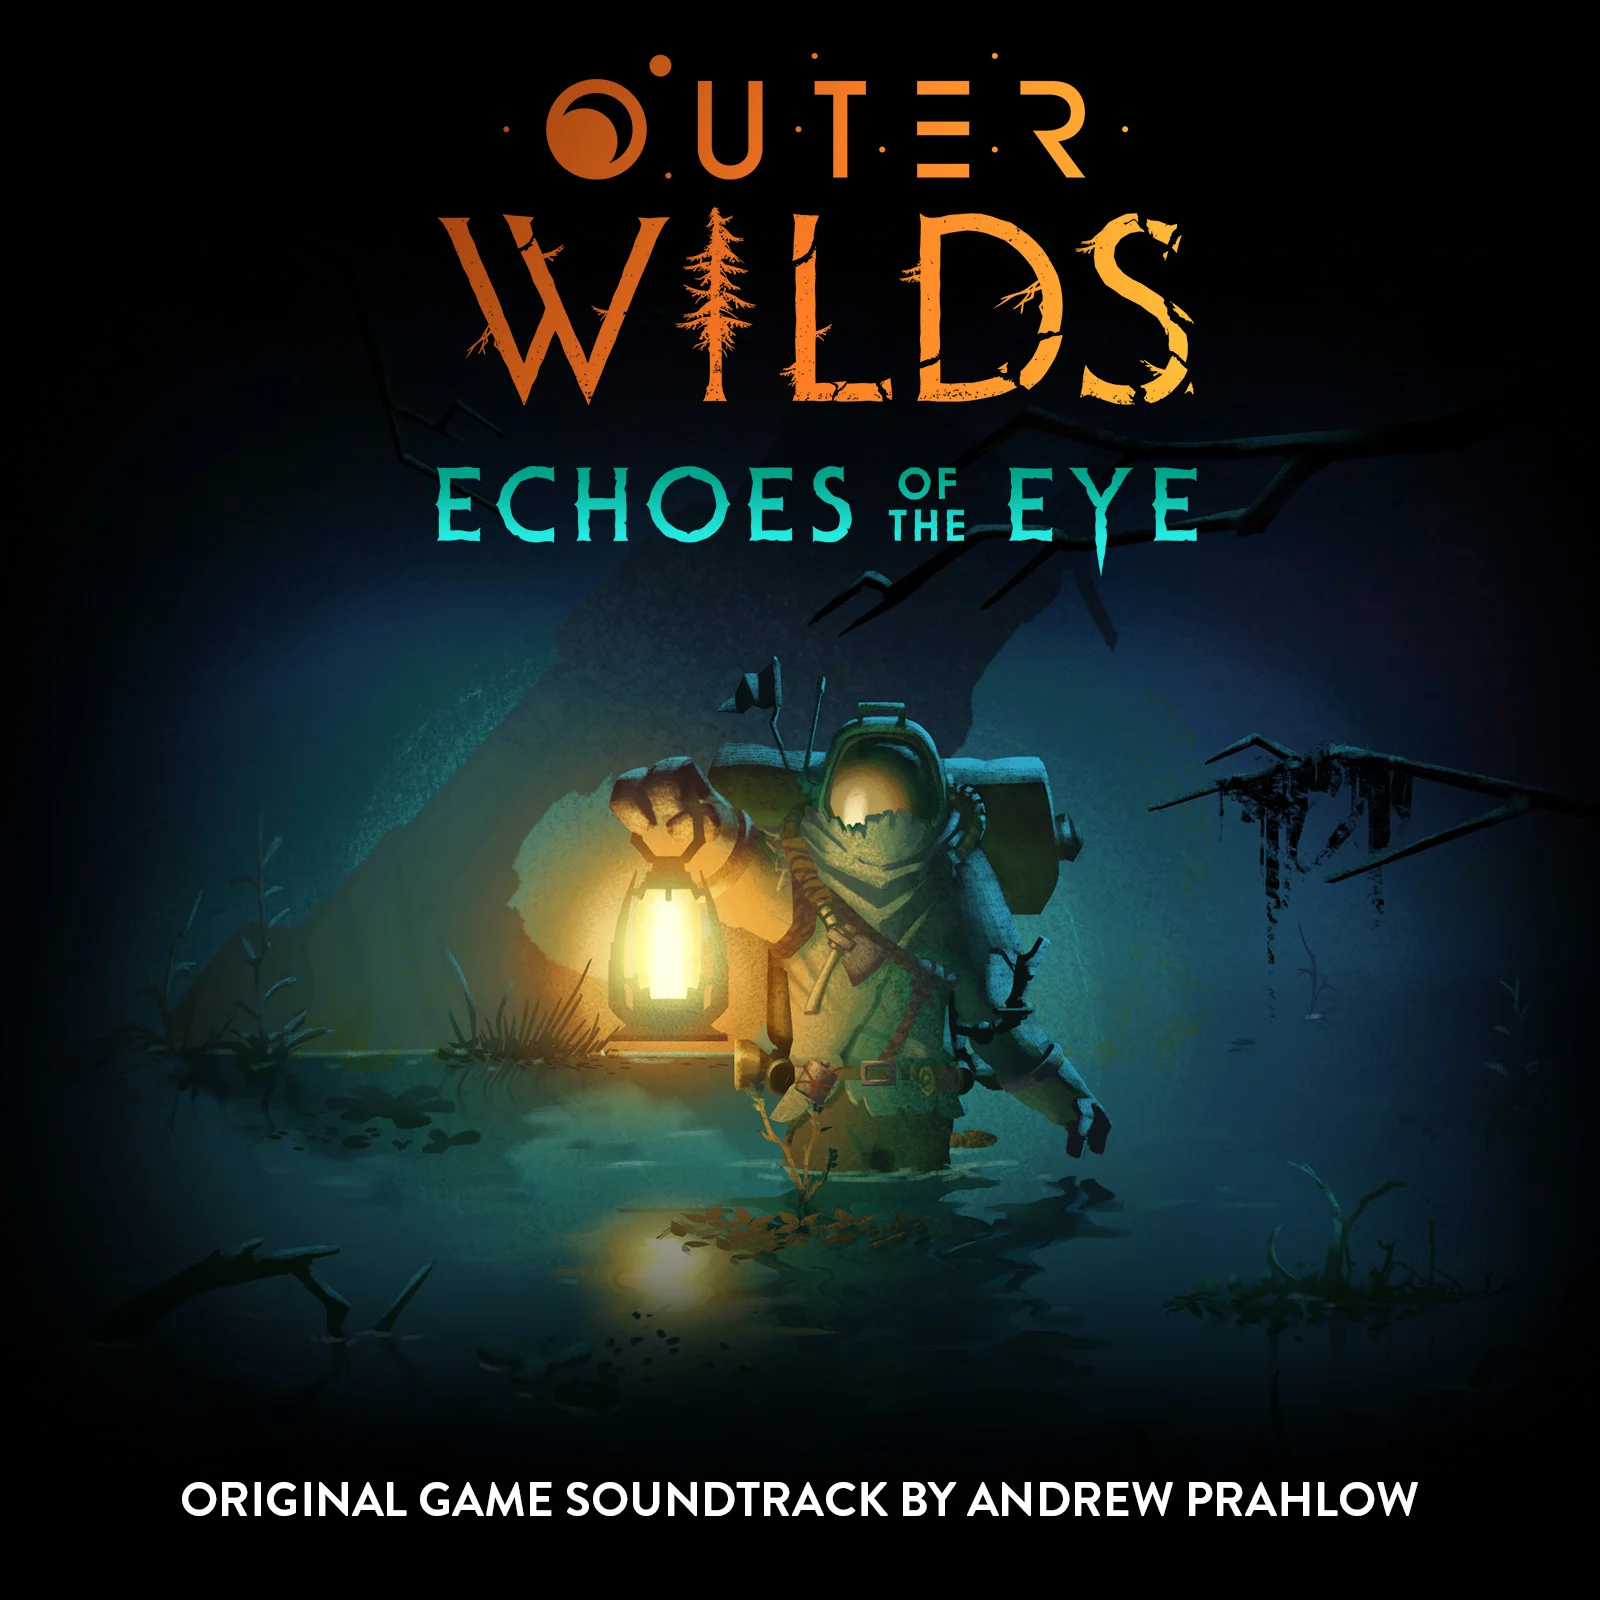
\includegraphics[width=0.8\textwidth]{Img/专辑图片.png}
    \caption{专辑图片}
\end{figure}

游戏最具辨识度的声音意象，是以木吉他、班卓琴、口哨等原声乐器构成的温暖音色。它们不像传统科幻作品中常见的宏大管弦乐或冰冷电子声那样强调技术感，而更接近营地、篝火和民谣。这样的选择与游戏的主角文明 Hearthian 的气质高度一致：他们虽然已经可以进行宇宙航行，却仍然保留着围坐篝火、手工造船、带着好奇心出发的朴素感。

这种音乐风格产生了一种重要的反差。玩家面对的是黑洞、量子天体、恒星坍缩和文明遗迹，但耳边最先出现的却是亲切、轻盈、带有手作感的旋律。它削弱了宇宙题材常见的冷峻距离，使太空探索不只是技术行为，而更像一次带着家乡记忆的远行。也正因为旋律具有“家”的质感，当玩家在陌生星球上听见熟悉主题时，孤独感会被短暂抚平，探索行为也被赋予了情感上的连续性。

游戏中每一位散布在不同星球上的旅人都有各自的乐器声部，例如班卓琴、鼓、长笛、口哨等。玩家可以使用信号镜追踪这些音乐信号，在宇宙空间中通过声音定位人物。这一机制让音乐直接进入了玩法层面：它不只是背景配乐，而成为导航线索和空间坐标。

更重要的是，这些独立声部共同构成了游戏的叙事隐喻。单独听某一位旅人的旋律时，它只是孤独的个人表达；当玩家逐渐找到所有旅人，理解他们在不同星球上的位置和故事后，这些旋律便像被重新编排一样，在玩家的记忆中合奏起来。游戏后期的音乐因此具有很强的回收感：它不是突然制造感动，而是把玩家在前期分散获得的声音经验重新组织，使“我曾经到过那里、见过他们、听过他们”的记忆在同一首音乐中汇合。

这种处理方式也呼应了《星际拓荒》的知识推进结构。玩家并不是沿着单一路线接受剧情，而是在碎片化探索中拼合真相。音乐同样以碎片的形式出现，再在关键时刻完成整体化呈现。由此，配乐成为叙事结构的镜像：每一个声部都是局部，每一次聆听都是线索，最终的合奏才显示出完整意义。

\subsection{循环时间与终局情绪}

二十二分钟循环是游戏最重要的时间框架，而音乐在其中承担了清晰的节奏提示功能。随着恒星接近超新星爆发，游戏会响起极具标志性的终末旋律。玩家在反复循环中逐渐形成条件反射：一旦听见这段音乐，就知道当前时间已经接近尾声，必须决定是继续冒险、抓紧验证线索，还是接受本轮探索即将结束。

这类音乐提示的高明之处在于，它没有用界面倒计时直接打断沉浸感，而是让时间压力以审美形式进入玩家感知。终末旋律既是机制提示，也是情绪推进。初次听见时，玩家可能只感到紧张和茫然；经历多次循环后，它又会带上熟悉、从容甚至仪式性的意味。音乐因此记录了玩家认知状态的变化：同一段旋律在不同阶段产生不同感受，正说明玩家已经从“被宇宙事件追赶的人”变成了“理解循环规律的人”。

《星际拓荒》的音乐具有明显的电影感，但这种电影感并不依赖持续铺满的配乐，而是来自对进入时机、音色密度和情绪留白的控制。游戏中的许多探索时刻保持相对安静，玩家听到的往往是推进器、呼吸声、环境声或星球本身的动态声响。正因为平时足够克制，当主题音乐在关键节点出现时，它才会显得格外清晰。

这种处理接近电影配乐中的“情绪转场”：音乐不是时时告诉玩家应当感受什么，而是在发现、接近真相或面对终局时，把已经积累的情绪推向可被感知的形态。重复出现的主题旋律也像电影中的主题动机，每一次回归都携带此前场景的记忆。玩家不是单纯听到一段好听的旋律，而是在旋律中重新经历自己探索过的星球、读过的碑文、见过的遗迹和理解过的牺牲。

在游戏结尾，音乐完成了从个人旅途到宇宙尺度叙事的转换。此前分散的旅人声部被重新召集，玩家通过一次近似篝火合奏的仪式，把漫长探索中建立的关系和记忆集中到同一场景中。这里的音乐不只是结局配乐，而是游戏主题的最终表达：宇宙终将走向终点，但曾经存在过的生命、好奇心、陪伴和理解并不会因此失去意义。

因此，《星际拓荒》的音乐赏析不能只停留在旋律是否动听的层面。它的价值在于把声音设计、叙事结构和玩家行为紧密结合起来：用民谣音色建立亲近感，用旅人乐器组织空间记忆，用终末主题提示循环时间，用主题回归完成情绪回收。音乐让玩家在一次次失败和重启中仍然感到旅程具有连续性，也让最终的宇宙终章不只是宏大的毁灭场面，而成为一次关于记忆、告别与新生的聆听经验。
